\documentclass{beamer}

\usepackage[utf8]{inputenc}
\usetheme{default}

\usepackage{siunitx}
\usepackage{enumerate}

\title{Simulation of MCP-PMT}
\author{Jakub Bucko}
\institute{Institute of Particle and Nuclear Physics, Charles University \and Supervisor: Dr. Tomáš Sýkora}
\date{27. 9. 2022}

\beamertemplatenavigationsymbolsempty
\setbeamertemplate{footline}{\vspace*{1mm}\hfill
\insertframenumber/\inserttotalframenumber\hfill\vspace*{1mm}}

\setbeamertemplate{footline}[frame number]

\setbeamerfont{footnote}{size=\tiny}

\begin{document}
    %\begin{frame}[plain]
    %    \titlepage
    %\end{frame}

    {\setbeamertemplate{footline}{}
    \begin{frame}[noframenumbering]
        \titlepage
    \end{frame}}


    \begin{frame}
        \frametitle{Microchannel plates}
        \begin{minipage}{0.4\linewidth}
            \includegraphics[scale=0.25]{"mcp.png"}
        \end{minipage}%
        \hspace{40pt}
        \begin{minipage}{0.4\linewidth}
            \includegraphics[scale=0.25]{"channel.png"}
        \end{minipage}

        %\begin{itemize}
          %  \item Model of ideal gain


           % \item Too simple: does not take into account emission angles, fringe fields, charge distribution, etc.
        %\end{itemize}

        \vspace{15pt}
        \begin{block}{Model of ideal gain}
            \vspace{-25pt}
            \begin{gather*}
                \delta = KV_c \\
                G = \delta^n = \left(\frac{KV_0}{4V\alpha^2}\right)^{\frac{4V\alpha^2}{V_0}}
            \end{gather*}
            Too simple: does not take into account emission angles, fringe fields, charge distribution, etc.
        \end{block}


        \let\thefootnote\relax\footnote{Original pictures from: Wiza, J. L. (1979). Microchannel plate detectors. Nucl. Instrum. Methods, 162(1-3), 587-601.}
    \end{frame}


    \begin{frame}
        \frametitle{Transmission line model}
        \begin{itemize}
            \item We consider TLM by L. Giudicotti
            \item In this model a channel is divided into parts represented by lumped component
            \item Kirshoff's laws are then used to derive the model equations
            \item Assumption: input pulse is shorter than typical charge recovery time $RC$,
                    but longer than the average transit time
        \end{itemize}
        \begin{minipage}{0.4\linewidth}
            \includegraphics[scale=0.8]{"TLM-scheme.pdf"}
        \end{minipage}
        \hspace{50pt}
        \begin{minipage}{0.4\linewidth}
            {\tiny Original paper: Giudicotti L. Nucl. Instrum. Methods Phys. Res. A, 659 (1)
(2011), pp. 336-347}

            \begin{itemize}
                \item We recalculated the derivation of the model equations
                \item Typo in (37): wrong sign in front of $(Q(x, t)/Qs)_n$
            \end{itemize}

        \end{minipage}

        \begin{equation*}
                g(x, t) = \exp{\{Gx + \int^x_0\ln{\left(1 + e^\frac{-t}{RC} \frac{Q_{W0}(t) + Q_0(t) - Q(x', t)}{Q_s} \right)} \text{d}x' \}}
        \end{equation*}
    \end{frame}

    \begin{frame}
        \frametitle{Recreation of results}
        \begin{minipage}{0.4\linewidth}
            \centering
            \textbf{Original plots}

            \includegraphics[scale=0.55]{"tlm-gain-orig.pdf"}
            \includegraphics[scale=0.55]{"tlm-gain-zoom-orig.pdf"}
            \includegraphics[scale=0.55]{"tlm-output-orig.pdf"}
        \end{minipage}
        \hspace{40pt}
        \begin{minipage}{0.4\linewidth}
            \centering
            \textbf{Recreation}

            \includegraphics[scale=0.225]{"g.pdf"}
            \includegraphics[scale=0.225]{"g_zoom.pdf"}
            \includegraphics[scale=0.225]{"oi.pdf"}
        \end{minipage}
    \end{frame}

    \begin{frame}
        \frametitle{Problem with the assumption}
        \begin{itemize}
            \item The average number of photoelectrons arriving to MCP-PMT is between 15 and 45
            \item Typical number of microchannels is $10^6 - 10^7$
            \item This means that there is less than one photoelectron per channel and we can expect
                    one photoelectron in a microchannel at maximum
            \item This corresponds to $i_0(t) = \delta(t) \Rightarrow$ signal length is shorter than
                    transition time
        \end{itemize}

    \end{frame}


    \begin{frame}
        \frametitle{Monte-Carlo simulation algorithm}

        \begin{enumerate}
            \item Calculate trajectory and collision energy of an initial electron
        \end{enumerate}

        \begin{center}
            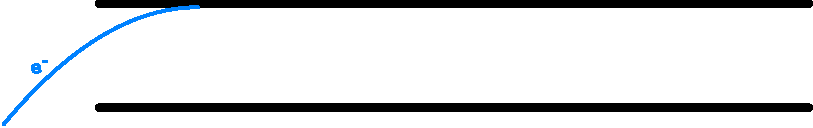
\includegraphics[width=\linewidth]{mc1.pdf}
        \end{center}
    \end{frame}

    \begin{frame}
        \frametitle{Monte-Carlo simulation algorithm}
        \begin{enumerate}[2.]
            \item From the collision energy, calculate the number of secondary electrons using some secondary emission function
        \end{enumerate}

        \begin{center}
            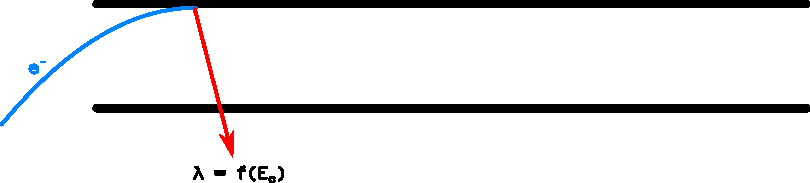
\includegraphics[width=\linewidth]{mc2.pdf}
        \end{center}
    \end{frame}

    \begin{frame}
        \frametitle{Monte-Carlo simulation algorithm}
        \begin{enumerate}[3.]
            \item We use this value as the mean value of Poisson distribution and generate the random number of secondary electrons
        \end{enumerate}

        \begin{center}
            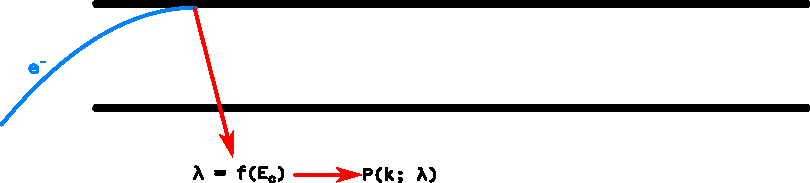
\includegraphics[width=\linewidth]{mc3.pdf}
        \end{center}
    \end{frame}

     \begin{frame}
        \frametitle{Monte-Carlo simulation algorithm}
        \begin{enumerate}[4.]
            \item Assign random initial angles and energies to secondary electrons
        \end{enumerate}

        \begin{center}
            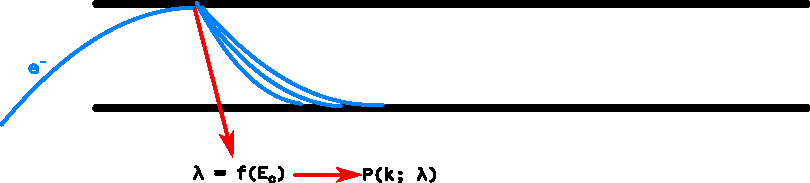
\includegraphics[width=\linewidth]{mc4.pdf}
        \end{center}
    \end{frame}

    \begin{frame}
        \frametitle{Monte-Carlo simulation algorithm}
        \begin{enumerate}[5.]
            \item Repeat for every secondary electron
        \end{enumerate}

        \begin{center}
            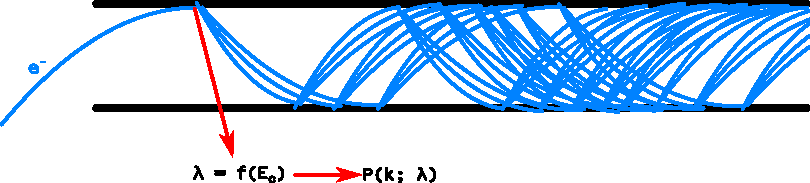
\includegraphics[width=\linewidth]{mc5.pdf}
        \end{center}
    \end{frame}


    \begin{frame}
        \frametitle{Outlook}

        \begin{itemize}
            \item Contact L. Giudicotti and discuss with him the problem of the assumption
            \item Improve the TLM simulation
            \item Work towards full Monte-Carlo simulation
        \end{itemize}

    \end{frame}



\end{document}
